\begin{theo}[Magnetische velden]{Magnetische velden}
    Net zoals we rondom een elektrische lading een elektrisch veld hebben gedefinieerd, kunnen we rond een magneet een magnetisch veld
    $\Vec{B}$ definiëren. Magnetische veldlijnen op tekeningen hebben dusdanig ook dezelfde eigenschappen als elektrische veldlijnen, namelijk

    \begin{minipage}{.7\textwidth}
        \begin{itemize}
            \item de richting van het magnetische veld is tangentieel met de magnetische veldlijnen
            \item de hoeveelheid magnetische veldlijnen per oppervlakte duidt op het sterkte van het magnetische veld
        \end{itemize}

    \end{minipage}
    \begin{minipage}{.24\textwidth}
        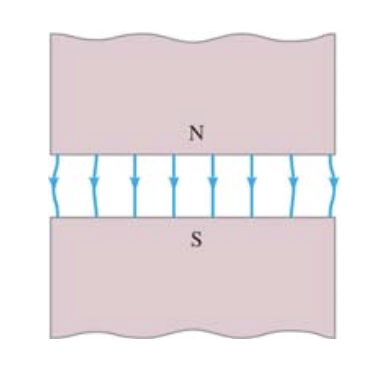
\includegraphics[scale = 0.52]{Images/Magnetisme/HomogeenMagnetischVeld}
    \end{minipage}

    \noindent Elektrische stroom \textbf{produceert} een magnetisch veld. Een niet-magnetische, geleidende draad is dus wel magnetisch als we er stroom op zetten.
    Om de richting van het magnetisch veld te weten, kunnen we \textbf{rechterhandregel 1} (zie Samenvatting 1) toepassen.

%    \begin{minipage}{.75\textwidth}
%        "Pak de draad vast met je rechterhand en steek je duim uit in
%        de richting van de conventionele stroomzin en vouw je vingers dicht in de richting van het magnetische veld."
%    \end{minipage}
%    \begin{minipage}{.21\textwidth}
%        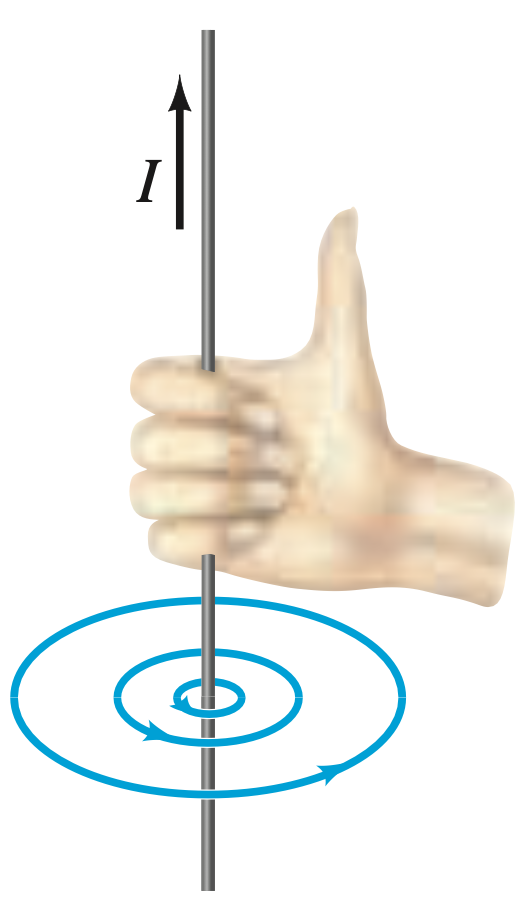
\includegraphics[scale = 0.2]{Images/Magnetisme/Rechterhandregel}
%    \end{minipage}

\end{theo}

%\begin{app}[Elekrtische stroom]{Elekrtische stroom}
%    Elektrische stroom \textbf{produceert} een magnetisch veld. Een niet-magnetische, geleidende draad is dus wel magnetisch als we er stroom op zetten.
%    Om de richting van het magnetisch veld te weten, kunnen we de \textbf{rechterhandregel} toepassen:
%
%    \begin{minipage}{.8\textwidth}
%        pak de draad vast met je rechterhand en steek je duim uit in
%        de richting van de conventionele stroomzin en vouw je vingers dicht in de richting van het magnetische veld.
%    \end{minipage}
%    \begin{minipage}{.16\textwidth}
%        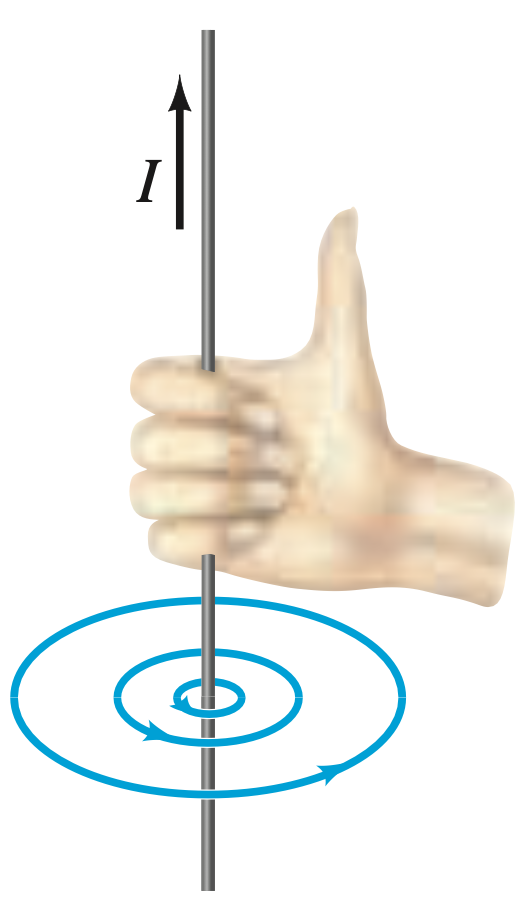
\includegraphics[scale = 0.2]{Images/Magnetisme/Rechterhandregel}
%    \end{minipage}
%\end{app}

\begin{theo}[Magnetische kracht]{Magnetische kracht}
    De relatie tussen de magnetische kracht $\Vec{F}$ van een draad met stroom $I$ en het magnetisch veld $\Vec{B}$ kan geschreven worden als een vector product
    \begin{equation*}
        d\Vec{F}= Id\Vec{\ell} \times \Vec{B}
    \end{equation*}
    waarbij $d\Vec{F}$ een infinitesimale kracht op een infinitesimale lengte $d\Vec{\ell}$ van de draad in het magnetische veld.
    \begin{center}
        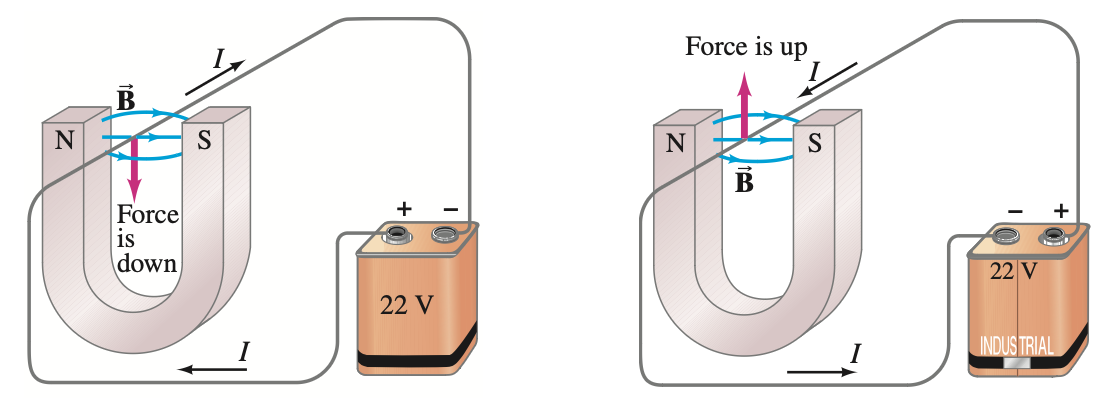
\includegraphics[scale = 0.45]{Images/Magnetisme/MagnetischeKracht}
    \end{center}
    \begin{minipage}{.75\textwidth}
        Als het veld homogeen is, dan zal elk infinitesimaal deeltje $d\Vec{\ell}$ dezelfde hoek maken met het magnetische veld $\Vec{B}$.
        Hieruit volgt dan de formule:
        \begin{equation*}
            \Vec{F} = I\Vec{\ell} \times \Vec{B}
        \end{equation*}
    \end{minipage}
    \begin{minipage}{.21\textwidth}
        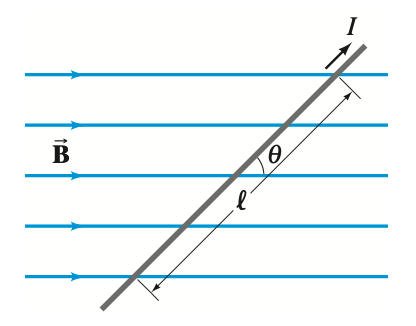
\includegraphics[scale = 0.25]{Images/Magnetisme/DraadHomogeenVeld}
    \end{minipage}
\end{theo}

%\begin{app}[Magnetische kracht in een homogeen veld]{Magnetische kracht in een homogeen veld}
%    \vspace{-0.5cm}
%    \begin{minipage}{.75\textwidth}
%        Als het veld homogeen is, dan zal elk infinitesimaal deeltje $d\Vec{\ell}$ dezelfde hoek maken met het magnetische veld $\Vec{B}$.
%        Hieruit volgt dan de formule:
%        \begin{equation*}
%            \Vec{F} = I\Vec{\ell} \times \Vec{B}
%        \end{equation*}
%    \end{minipage}
%    \begin{minipage}{.21\textwidth}
%        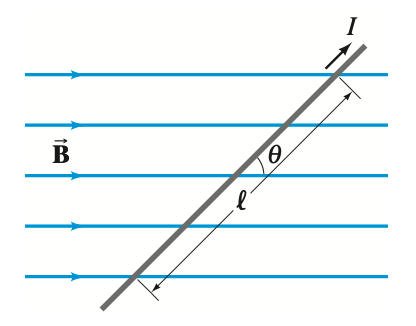
\includegraphics[scale = 0.25]{Images/Magnetisme/DraadHomogeenVeld}
%    \end{minipage}
%\end{app}

%\begin{ex}[Willekeurige stroomvoerende geleider in een homogeen magnetisch veld]{Willekeurige stroomvoerende geleider in een homogeen magnetisch veld}
%    \begin{minipage}{.6\textwidth}
%        \vspace{-0.5cm}
%        \begin{align*}
%            \Vec{F} &= I\int_a^{b}d\Vec{l} \times \Vec{B} \\
%            &= I(\int_a^{b}d\Vec{l} \times \Vec{B}) \quad \text{(B is homogeen)} \\
%            &= I(\Vec{L} \times \Vec{B})
%        \end{align*}
%    \end{minipage}
%    \begin{minipage}{.36\textwidth}
%        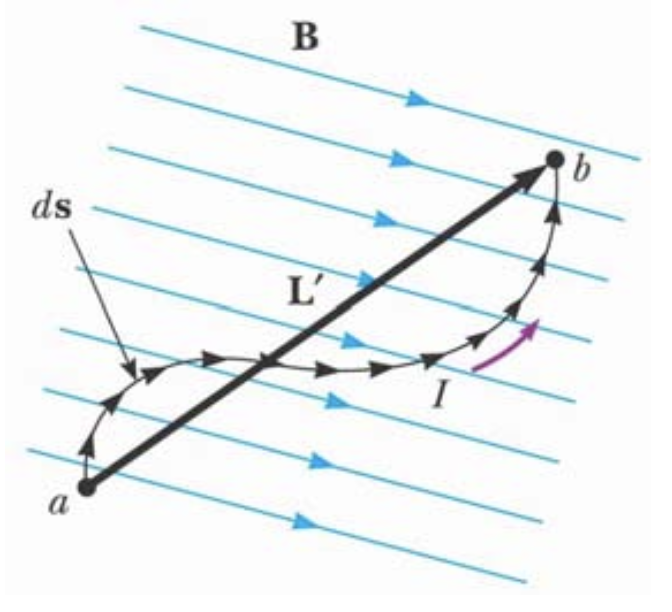
\includegraphics[scale = 0.35]{Images/Magnetisme/StroomvoerendeGeleiderHomogeenMagnetischVeld}
%    \end{minipage}
%\end{ex}


\newpage

\begin{theo}[Magnetische kracht op een bewegende lading]{Magnetische kracht op een bewegende lading}
    Elektrische stroom is een verzameling van N bewegende ladingen, we kunnen de definitie van magnetische kracht dus ook anders schrijven:
    \begin{equation*}
        \Vec{F} = I\Vec{\ell} \times \Vec{B} = Nq\Vec{v} \times \Vec{B}
    \end{equation*}
    sinds $I = \tfrac{Nq}{t}$ en $\Vec{\ell} = \Vec{v}t$.
\end{theo}

\begin{vrg}[Verschillen tussen elektrische en magnetische kracht]{Verschillen tussen elektrische en magnetische kracht}
    \vspace{-0.3cm}
    \def\arraystretch{2}
    \hspace{-0.35cm}
    \begin{tabular}{c|c}
        Elektrische kracht: $\Vec{F} = q\Vec{E}$ & Magnetische kracht: $\Vec{F} = q\Vec{v} \times \Vec{B}$ \\ \hline
        in de \textbf{richting} van het elektrsich veld & \textbf{loodrecht} op het magnetische veld \\
        werkt op een \textbf{lading} & werkt op een \textbf{bewegende lading} \\
        levert \textbf{arbeid} bij de verplaatsing van de lading & levert \textbf{geen arbeid} bij de verplaatsing van de lading \\
    \end{tabular}
\end{vrg}

\begin{app}[Bewegende lading in een vlak loodrecht op magnetisch veld]{Bewegende lading in een vlak loodrecht op magnetisch veld}
    \begin{minipage}{.67\textwidth}
        Het pad van een bewegende lading in een vlak loodrecht op het magnetisch veld is cirkelvormig.
        De kracht zal altijd loodrecht zijn op de snelheid, dus de lading zal cirkelvormig bewegen met
        centripetale versnelling:
        \begin{equation*}
            a = \dfrac{v^2}{r}.
        \end{equation*}
        De periode heeft de volgende formule:
        \begin{equation*}
            T = \dfrac{2\pi r}{v} = \dfrac{2\pi m}{qB} = \dfrac{1}{f}
        \end{equation*}
        sinds $r = \tfrac{mv}{qB}$.
    \end{minipage}
    \begin{minipage}{.29\textwidth}
        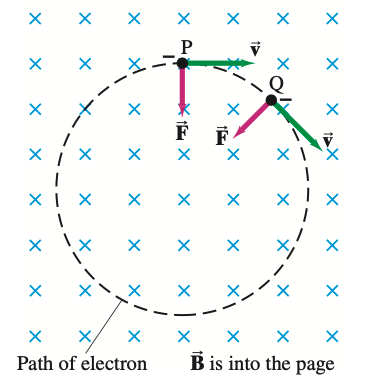
\includegraphics[scale = 0.35]{Images/Magnetisme/CirkelvormigeBewegingMagentischVeld}
    \end{minipage}
\end{app}

\begin{theo}[Magnetisch dipool moment]{Magnetisch dipool moment]}
    Wanneer een lading stroom door een gesloten kring in een extern magnetisch veld, dan kan de magnetische kracht torsie veroorzaken.
    Stroom vloeit door de rechthoekige kring (zie figuur a), waarvan we aannemen dat het parrallel is met het veld $\Vec{B}$.
    Het veld oefent noch een kracht, noch een krachtmoment uit op de horizontale delen; hier is $\sin(\theta) = 0$. Het veld oefent wel een kracht uit op de verticale delen
    (hiervan geeft figuur b een bovenaanzicht), we noemen deze krachten $\Vec{F_1}$ en $\Vec{F_2}$. Deze krachten zorgen voor een netto krachtmoment:
    \begin{equation*}
        \tau = IaB\dfrac{b}{2} + IaB\dfrac{b}{2} = IabB = IAB
    \end{equation*}
    waarbij $A = ab$ de oppervlakte van de spoel.

    \newpage

    \hspace{-0.5cm}\begin{minipage}{0.76\textwidth}
        Als de spoel $N$ kringen heeft en een hoek $\theta$ maakt met het magnetisch veld (zie figuur c),
        dan is de stroom $NI$ en volgt:
        \begin{equation}\label{eq:1}
            \tau = NIAB\sin(\theta)
        \end{equation}
        want de krachten blijven gelijk, maar de krachtarmen verkleint.
        Het \textbf{magnetisch dipool moment} $\Vec{\mu}$ wordt als volgt gedefinieerd"
        \begin{equation*}
            \Vec{\mu} = NI\Vec{A}
        \end{equation*}
        waarbij de ricthing van $\Vec{A}$ loodrecht is op het vlak van de spoel. Hiermee kunnen we (\ref{eq:1}) vectorieel schrijven:
        \begin{equation*}
            \Vec{\tau} = NI\Vec{A} \times \Vec{B} = \Vec{\mu} \times \Vec{B}
        \end{equation*}
        De potentiële energie U kunnen we dan als volgt berekenen
        \begin{equation*}
            U = \int_0^{\tfrac{\pi}{2}} \tau d\theta = \int_0^{\tfrac{\pi}{2}} NIAB\sin(\theta) d\theta = -\mu B\cos(\theta) = -\Vec{\mu} \cdot \Vec{B}
        \end{equation*}
        wat ook logisch is sinds we dit kunnen vergelijkigen met het elektrisch dipool moment (zie 10.4).
    \end{minipage}
    \begin{minipage}{.2\textwidth}
        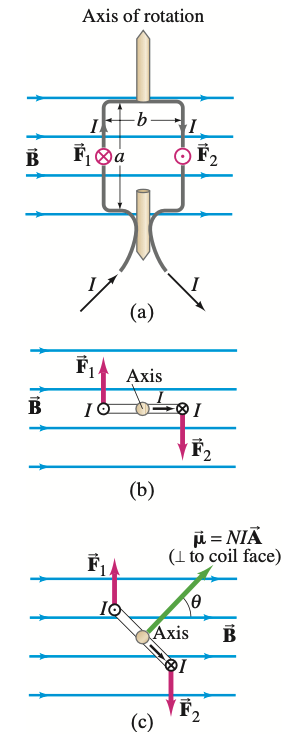
\includegraphics[scale = 0.35]{Images/Magnetisme/MagnetischDipoolMoment}
    \end{minipage}
    \vspace{0.2cm}
\end{theo}

\begin{summ}[Rechterhandregels]{Rechterhandregels}
    \centering
    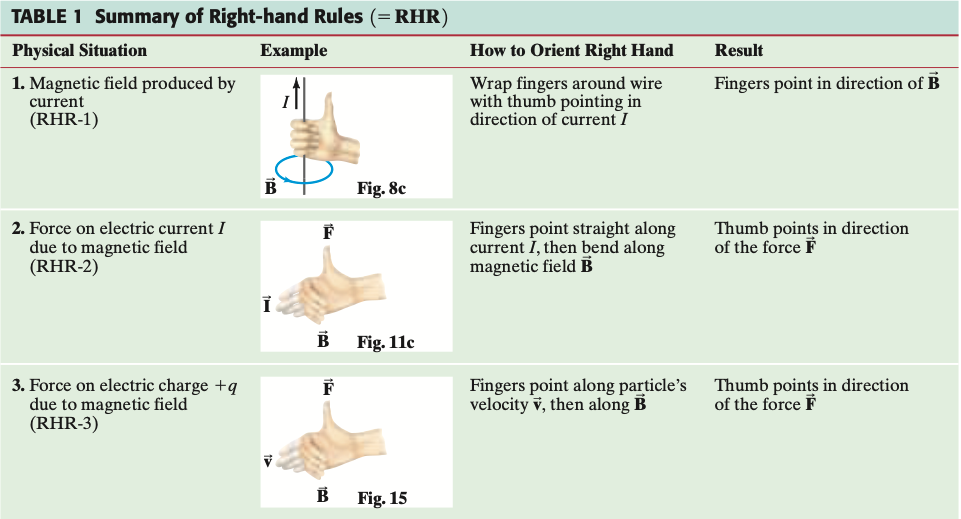
\includegraphics[scale=0.45]{Images/Magnetisme/RechterhandRegels}
\end{summ}

